% ============================================================
% Continuation from ch3 (Forces, Shell Theorem)
% Pages 12–38: Atwood machine, polar coordinates kinematics,
%   friction, Newton's laws, spring force, pendulum, adding
%   springs, viscosity, and recitation problems.
% ============================================================

\section{Inclined Plane (continued)}

\begin{figure}[H]
\begin{center}
\begin{tikzpicture}[scale=1.1, >=Stealth]
  % Inclined plane triangle
  \draw[thick] (0,0) -- (4,0) -- (4,2.3) -- cycle;
  \node at (0.7,0.18) {$\theta$};
  \draw (0.55,0) arc[start angle=0, end angle=30, radius=0.55];
  % Block
  \def\bx{1.6}\def\by{0.92}
  \begin{scope}[rotate around={30:(\bx,\by)}]
    \fill[gray!30] (\bx-0.3,\by-0.3) rectangle (\bx+0.3,\by+0.3);
    \draw[thick] (\bx-0.3,\by-0.3) rectangle (\bx+0.3,\by+0.3);
  \end{scope}
  % Weight arrow (downward)
  \draw[->,thick,blue] (1.6,0.92) -- (1.6,-0.5) node[below]{$\vect{w}=m\vect{g}$};
  % Normal arrow (perpendicular to slope)
  \draw[->,thick,red] (1.6,0.92) -- ++(150:1.1) node[above left]{$\vect{N}$};
  % Acceleration along slope
  \draw[->,thick,ForestGreen] (1.6,0.92) -- ++(30:1.1) node[right]{$\vect{a}$};
\end{tikzpicture}
\end{center}
\caption{Block on a frictionless inclined plane at angle $\theta$; normal force $\vect{N}$ perpendicular to surface, weight $\vect{w} = m\vect{g}$ downward.}
\label{fig:inclined_plane}
\end{figure}

Newton's second law $\vect{N} + \vect{w} = m\vect{a}$, projected onto axes along and perpendicular to the slope:

\begin{align*}
x&: \quad w\sin\theta = ma \implies mg\sin\theta = ma \implies a = g\sin\theta \\
y&: \quad N - w\cos\theta = 0
\end{align*}

\textbf{Limiting cases:} $\theta = 0$ (flat, $a=0$) \checkmark \quad $\theta = \tfrac{\pi}{2}$ (free fall, $a=g$) \checkmark

% ============================================================
\section{Atwood Machine}
% ============================================================

\begin{figure}[H]
\begin{center}
\begin{tikzpicture}[scale=0.9, >=Stealth]
  % Pulley support and axle
  \draw[thick] (-0.1,3.2) -- (0.1,3.2);
  \draw[thick] (0,3.2) -- (0,2.8);
  % Pulley circle
  \draw[thick] (0,2.5) circle[radius=0.3];
  \fill[gray!40] (0,2.5) circle[radius=0.08];
  % Left rope and mass m1
  \draw[thick] (-0.3,2.5) -- (-0.3,1.2);
  \fill[gray!50] (-0.55,0.8) rectangle (-0.05,1.2);
  \draw[thick] (-0.55,0.8) rectangle (-0.05,1.2);
  \node at (-0.3,1.0) {$m_1$};
  \draw[->,thick,blue] (-0.3,0.8) -- (-0.3,0.1) node[below]{$w_1$};
  \draw[->,thick,red] (-0.3,1.2) -- (-0.3,1.9) node[right]{$T_1$};
  % Right rope and mass m2
  \draw[thick] (0.3,2.5) -- (0.3,0.7);
  \fill[gray!50] (0.05,0.3) rectangle (0.55,0.7);
  \draw[thick] (0.05,0.3) rectangle (0.55,0.7);
  \node at (0.3,0.5) {$m_2$};
  \draw[->,thick,blue] (0.3,0.3) -- (0.3,-0.3) node[below]{$w_2$};
  \draw[->,thick,red] (0.3,0.7) -- (0.3,1.4) node[right]{$T_2$};
  % Ceiling
  \fill[pattern=north east lines] (-0.5,3.2) rectangle (0.5,3.4);
  \draw[thick] (-0.5,3.2) -- (0.5,3.2);
\end{tikzpicture}
\end{center}
\caption{Atwood machine: two masses $m_1$ and $m_2$ connected by an inextensible rope over a pulley of radius $R$. Tensions $T_1$, $T_2$ act upward on each mass; weights $w_1$, $w_2$ act downward.}
\label{fig:atwood}
\end{figure}

\begin{example}[Atwood Machine]
Two masses $m_1$ and $m_2$ hang from either end of a rope over a fixed pulley. Find the acceleration.

\textbf{System \{1\}:} tension $T_1$ upward, weight $w_1 = m_1 g$ downward.
\[
\vect{T}_1 + \vect{w}_1 = m_1 \vect{a}_1 \implies T_1 - m_1 g = m_1 \ddot{y}_1
\]

\textbf{System \{2\}:} tension $T_2$ upward, weight $w_2 = m_2 g$ downward.
\[
T_2 - m_2 g = m_2 \ddot{y}_2
\]

\textbf{Constraint} --- length of rope is constant $= \ell$:
\[
\ell = y_p - y_1 + y_p - y_2 + \pi R
\]
Differentiating twice:
\[
\dv{\ell}{t} = 0 = -\dot{y}_1 - \dot{y}_2 \implies 0 = -\dot{y}_1 - \dot{y}_2
\]

The tension of the rope should balance unless the rope is stretching, so $T_1 = T_2 \equiv T$.

\textbf{Putting everything together:}
\begin{align*}
T - m_1 g &= m_1 \ddot{y}_1 \\
T - m_2 g &= m_2 \ddot{y}_2
\end{align*}

Using the constraint $\ddot{y}_2 = -\ddot{y}_1$, subtract the two equations:
\begin{align*}
(T - m_1 g) - (T - m_2 g) &= m_1 \ddot{y}_1 + m_2 \ddot{y}_1 \\
(-m_1 + m_2)g &= (m_1 + m_2)\ddot{y}_1
\end{align*}

\begin{formula}[Atwood Machine Acceleration]
\[
\ddot{y}_1 = \frac{(-m_1 + m_2)\,g}{m_1 + m_2} = \frac{(m_2 - m_1)\,g}{m_1 + m_2}
\]
\end{formula}

\textbf{Check:} if $m_1 \gg m_2 \Rightarrow \ddot{y}_1 = -g$ (mass 1 falls freely). \checkmark
\end{example}

% ============================================================
\section{Polar Coordinates Example}
% ============================================================

\begin{example}[Rotating Table with Hanging Mass]
A object $A$ rotates at angular speed $\omega_0$ at radius $r_0$ on a frictionless horizontal table. It is connected through a hole in the table by a string to a hanging mass $B$. What is the acceleration of $A$ after $B$ is released?

\begin{figure}[H]\centering
\caption{Mass $A$ on a rotating table connected via a string through the table centre to hanging mass $B$. The string length $L = r + y_B = \text{const}$.}
\end{figure}

\textbf{System \{A\}:} Only horizontal tension $T$ acts (normal $N$ and weight $w_A$ cancel vertically).
\[
\vect{T} = m_A \vect{a}_A, \qquad
\vect{a}_A = (\ddot{r} - r\dot{\theta}^2)\,\rhat + (r\ddot{\theta} + 2\dot{r}\dot{\theta})\,\tthat
\]

Projecting:
\begin{align*}
\rhat&: \quad -T = m_A(\ddot{r} - r\dot{\theta}^2) \tag{1} \\
\tthat&: \quad 0 = m_A(r\ddot{\theta} + 2\dot{r}\dot{\theta}) \tag{2}
\end{align*}

\textbf{System \{B\}:} weight $m_B g$ downward, tension $T$ upward.
\[
m_B g - T = m_B \ddot{y}_B \tag{3}
\]

\textbf{Constraint:} $L = r + y_B = \text{const}$, so differentiating:
\[
\dot{r} = -\dot{y}_B \implies \ddot{r} = -\ddot{y}_B \tag{4}
\]

\textbf{Initial conditions:} $r = r_0$, $\dot{\theta} = \omega_0$.

From (1): $T = -m_A(\ddot{r} - r\dot{\theta}^2) = m_A(r\dot{\theta}^2 - \ddot{r})$.

Substituting into (3) with $\ddot{y}_B = -\ddot{r}$:
\begin{align*}
m_B g - m_A(r\dot{\theta}^2 - \ddot{r}) &= m_B(-\ddot{r}) \\
m_B g + m_A \ddot{r} - m_A r\dot{\theta}^2 &= -m_B \ddot{r} \\
m_B g + m_B \ddot{r} + m_A \ddot{r} &= m_A r\dot{\theta}^2 \\
\ddot{r}(m_A + m_B) &= m_A r\dot{\theta}^2 - m_B g
\end{align*}

\begin{formula}[Polar Constraint System]
\[
\ddot{r} = \frac{m_A r\dot{\theta}^2 - m_B g}{m_A + m_B}
\]
\end{formula}
\end{example}

% ============================================================
\chapter{Forces}
% ============================================================

\section{Friction}

\begin{definition}[Friction]
Friction arises when the surface of one body moves (or tends to move) across another. It:
\begin{itemize}
  \item opposes motion,
  \item is independent of the area of the object,
  \item acts proportional to the normal force $N$.
\end{itemize}
\[
f = \mu N \qquad (\mu \text{ a unitless constant})
\]
\end{definition}

\subsection{Types of Friction}

There are two coefficients: $\mu_{\text{static}}$ and $\mu_{\text{kinetic}}$.

\begin{fact}[Static Friction]
Bodies are \emph{not} in relative motion:
\[
0 \le f_s \le \mu_s N
\]
Direction: opposes the motion the object \emph{would} have if it were moving.
\end{fact}

\begin{fact}[Kinetic Friction]
\[
f_k = \mu_k N
\]
Direction: opposite to the relative velocity.
\end{fact}

\textbf{Decision flowchart for friction:}
\begin{enumerate}
  \item Are the objects accelerating relative to each other?
    \begin{itemize}
      \item Yes $\Rightarrow f = \mu_k N$.
      \item No $\Rightarrow$ Are the objects just about to slip/not slip?
        \begin{itemize}
          \item Yes $\Rightarrow f = \mu_s N$.
          \item No $\Rightarrow$ don't assume anything about $f$; solve for it.
        \end{itemize}
    \end{itemize}
\end{enumerate}

\begin{example}[Block on Wedge with Friction]
A block of mass $m$ sits on a wedge at angle $\theta$. Forces: normal $N$, friction $f$, weight $mg$.

\begin{figure}[H]
\begin{center}
\begin{tikzpicture}[scale=1.0, >=Stealth]
  % Inclined wedge
  \draw[thick,fill=gray!10] (0,0) -- (3.5,0) -- (3.5,2.0) -- cycle;
  \node at (0.65,0.15) {$\theta$};
  \draw (0.55,0) arc[start angle=0, end angle=30, radius=0.55];
  % Block (rotated)
  \begin{scope}[rotate around={30:(1.5,0.86)}]
    \fill[gray!40] (1.2,0.6) rectangle (1.8,1.12);
    \draw[thick] (1.2,0.6) rectangle (1.8,1.12);
  \end{scope}
  \node at (1.65,0.9) {$m$};
  % Weight arrow
  \draw[->,thick,blue] (1.5,0.86) -- (1.5,-0.15) node[below]{$mg$};
  % Normal force (perpendicular to slope = direction 120 deg)
  \draw[->,thick,red] (1.5,0.86) -- ++(120:1.1) node[above]{$N$};
  % Friction force (up the slope = 30 deg direction)
  \draw[->,thick,ForestGreen] (1.5,0.86) -- ++(150:0.85) node[left]{$f$};
\end{tikzpicture}
\end{center}
\caption{Free-body diagram of block on inclined wedge at angle $\theta$: weight $mg$ downward, normal force $N$ perpendicular to surface, friction $f$ along the surface opposing motion.}
\label{fig:friction_wedge}
\end{figure}

\begin{align*}
x&: \quad mg\sin\theta - \mu F_N = m\ddot{x} \\
y&: \quad N - mg\cos\theta = 0 \implies N = mg\cos\theta
\end{align*}
\[
\therefore\quad \ddot{x} = g\sin\theta - \mu g\cos\theta
\]

\textbf{Maximum angle before sliding begins:}
\[
\theta_{\max} = \tan^{-1}(\mu)
\]
For different materials, the block starts sliding at different angles.
\end{example}


% ============================================================
\chapter{Dimensional Analysis and Order-of-Magnitude Estimates}
% ============================================================

\section{Dimensional Analysis}

\begin{definition}[Dimensional Analysis]
Shorthand solving using units alone. Used to check answers. \emph{NOT} to be confused with unit conversion.
\end{definition}

\begin{example}[Period of a Pendulum]
Relevant quantities: $\ell$ (length), $g$ (gravitational acceleration), $m$ (mass).
\[
[\ell] = L, \quad [g] = \frac{L}{T^2}, \quad [m] = M
\]

Assume $P = A\,\ell^x g^y m^z$. Then:
\[
T = A \cdot L^x \cdot \left(\frac{L}{T^2}\right)^y \cdot M^z = A\cdot L^{x+y} \cdot T^{-2y} \cdot M^z
\]

Matching exponents: $-2y = 1 \Rightarrow y = -\tfrac{1}{2}$; $x + y = 0 \Rightarrow x = \tfrac{1}{2}$; $z = 0$.

\[
\therefore\quad P = A\sqrt{\frac{\ell}{g}}
\]
\end{example}

\section{Order-of-Magnitude / Back-of-the-Envelope Estimates}

\begin{example}[Volume of Earth's Atmosphere]
\[
V_{\text{atmosphere}} \approx 4\pi R_\oplus^2 \cdot t
\]
where $t$ is the thickness of the atmosphere. Assume $t \approx 10^4\,\mathrm{m}$, $R_\oplus = 6\times 10^6\,\mathrm{m}$, and $t \ll R_\oplus$:
\[
\Rightarrow V \approx \boxed{4\times 10^{18}\,\mathrm{m}^3}
\]
\end{example}

\begin{example}[Terminal Velocity of a Raindrop]
Equation of motion with drag $F = -kv^2$:
\[
\dv{v}{t} = g - kv^2
\]
At terminal velocity $\dv{v}{t} = 0$:
\[
V_t \approx \sqrt{\frac{g}{k}}
\]
Dimensional check: $\left[\dv{v}{t}\right] = \dfrac{L}{T^2}$, $\dfrac{L}{T^2} - \left(\dfrac{1}{L}\right)\dfrac{L^2}{T^2}$ so $[k] = \dfrac{1}{L}$.

Order-of-magnitude estimate: $V_t \approx 5\,\mathrm{m/s}$.

What is $\kappa$?
\[
k = \frac{g}{V_t^2} \approx \frac{10\,\mathrm{m/s}^2}{(5\,\mathrm{m/s})^2} \approx 0.4\,\mathrm{m}^{-1}
\]
\end{example}

\section{Gravity (Newton's Law of Gravitation)}

\begin{figure}[H]\centering
\caption{Two masses $M_a$ and $M_b$ separated by distance $r$; gravitational force $\vect{F}_{ba}$ on $b$ from $a$ directed toward $a$, and $\vect{F}_{ab}$ directed toward $b$.}
\end{figure}

\begin{formula}[Newton's Law of Gravitation]
\[
\left|\vect{F}_{b/a}\right| = \frac{G m_a m_b}{r^2}
\]
Dimensions of $G$: $\dfrac{M \cdot L/T^2 \cdot L^2}{M^2} = \dfrac{L^3}{M \cdot T^2}$, i.e.\ $\mathrm{m}^3\,\mathrm{kg}^{-1}\,\mathrm{s}^{-2}$.
\end{formula}

Gravity is a \textbf{central} force, so:
\[
\vect{F}_{BA} = -\frac{GM_A M_B}{r^2}\,\rhat
\]

\subsection{Shell Theorem Results}

For a uniform spherical shell of mass $M$ and radius $R$:
\begin{align*}
r < R&: \quad \vect{F} = \vect{0} \\
r \ge R&: \quad \vect{F} = -\frac{GmM}{r^2}\,\rhat
\end{align*}

\subsection{Additional Notes on Gravity}

For acceleration due to gravity $g$, $\Delta g$ can be calculated as:
\[
\Delta g = g(R_e + h) - g(R_e) \approx h\,\dv{g}{r} = -\frac{2GM_e\,h}{R_e^3} = -2g\frac{h}{R_e}
\]

\textbf{Weight} at the surface of the Earth:
\[
W = -\frac{GM_e m}{R_e^2}\,\rhat = mg
\]

\section{Equivalence Principle}

\begin{fact}[Equivalence Principle]
Acceleration due to gravity is independent of mass.
\end{fact}

\section{Electrostatic Force}

\begin{formula}[Coulomb's Law]
\[
\vect{F}_{ba} = k\frac{q_1 q_2}{r^2}\,\hat{r}_{ba}, \qquad E = k\frac{q}{r^2}\,\rhat
\]
\end{formula}

\section{Phenomenological Forces}

\subsection{Contact Forces}

Forces transmitted between bodies by short-range interactions.

\subsection{Tension}

\begin{definition}[Tension]
Force due to a string's resistance to increasing length. You can imagine a chain of molecules that pull on each other as a string.

\begin{figure}[H]\centering
\caption{Each segment of the string transmits force $F'$ inward on both sides; applied force $F$ at one end. The tension is the same throughout a massless, inextensible string.}
\end{figure}
\end{definition}


% ============================================================
\chapter{Spring Force and Simple Harmonic Motion}
% ============================================================

\section{Hooke's Law}

\begin{formula}[Hooke's Law]
\[
\vect{F} = -k(\vect{x} - \vect{x}_0)
\]
where $x_0$ is the length of the spring at equilibrium.
\end{formula}

\begin{figure}[H]
\begin{center}
\begin{tikzpicture}[scale=1.0, >=Stealth]
  % Wall
  \fill[pattern=north east lines] (-0.2,-0.4) rectangle (0,0.4);
  \draw[thick] (0,-0.4) -- (0,0.4);
  % Spring (zigzag)
  \draw[thick, decorate, decoration={zigzag, segment length=6pt, amplitude=4pt}]
    (0,0) -- (2.5,0);
  % Mass block
  \fill[gray!40] (2.5,-0.3) rectangle (3.1,0.3);
  \draw[thick] (2.5,-0.3) rectangle (3.1,0.3);
  \node at (2.8,0) {$m$};
  % Equilibrium marker
  \draw[dashed] (2.8,-0.5) -- (2.8,-0.85);
  \node[below] at (2.8,-0.85) {$x_0$};
  % Spring force arrow
  \draw[->,thick,red] (3.1,0) -- (3.9,0) node[right]{$x$};
  \draw[->,thick,blue] (2.5,0) -- (1.7,0) node[left]{$F_s$};
  % Ground line
  \draw[thick] (-0.2,-0.4) -- (4.0,-0.4);
\end{tikzpicture}
\end{center}
\caption{Mass on a spring: equilibrium position $x_0$, displacement $x$ to the right, restoring spring force $F_s = -k(x-x_0)$ directed back toward equilibrium.}
\label{fig:spring_mass}
\end{figure}

Equation of motion (1D):
\[
\vect{F} = m\vect{a} \implies m\ddot{x} = -k(x - x_0)
\]

\subsection{Solving the Equation of Motion}

Introduce change of variables $\Delta x = x - x_0$, so $\Delta \ddot{x} = \ddot{x}$:
\[
\Delta\ddot{x} = -\frac{k}{m}\Delta x \qquad \textbf{(extremely important)}
\]

This is a second-order ODE, requiring 2 sets of initial conditions.

\textbf{Guess a solution and check:}
\[
y(t) = A\cos(\omega t + \phi_0)
\]
\[
\dot{y}(t) = -\omega A\sin(\omega t + \phi_0)
\]
\[
\ddot{y}(t) = -A\omega^2\cos(\omega t + \phi_0)
\]

Substituting:
\[
-A\omega^2\cos(\omega t + \phi_0) = -\frac{k}{m}A\cos(\omega t + \phi_0)
\]

\begin{formula}[Angular Frequency of SHM]
\[
\omega^2 = \frac{k}{m} \implies \omega = \sqrt{\frac{k}{m}}
\]
\end{formula}

\textbf{Interpretation of parameters:}
\begin{itemize}
  \item $A$: Amplitude — maximum distance it will travel.
  \item $\phi_0$: Phase — initial displacement; where did my system start at $t = 0$.
  \item $\omega$: Angular frequency — tells us about the period.
\end{itemize}

\begin{figure}[H]
\begin{center}
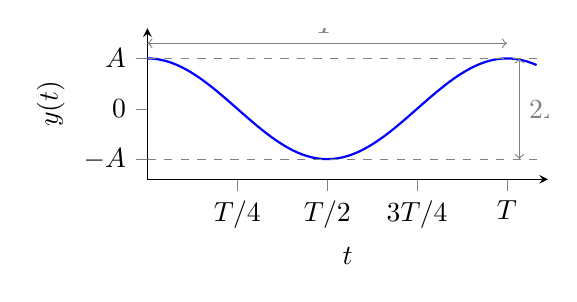
\begin{tikzpicture}
\begin{axis}[
  width=0.55\textwidth, height=3.5cm,
  xlabel={$t$}, ylabel={$y(t)$},
  xmin=0, xmax=7, ymin=-1.4, ymax=1.6,
  xtick={1.5708, 3.1416, 4.7124, 6.2832},
  xticklabels={$T/4$, $T/2$, $3T/4$, $T$},
  ytick={-1,0,1},
  yticklabels={$-A$, $0$, $A$},
  axis lines=left,
  tick align=outside,
  samples=200,
]
  \addplot[thick, blue, domain=0:6.8] {cos(deg(x))};
  % Amplitude annotations
  \draw[dashed, gray] (axis cs:0,1) -- (axis cs:6.8,1);
  \draw[dashed, gray] (axis cs:0,-1) -- (axis cs:6.8,-1);
  \draw[<->,gray] (axis cs:6.5,-1) -- (axis cs:6.5,1) node[midway,right]{$2A$};
  % Period brace
  \draw[<->,gray] (axis cs:0,1.3) -- (axis cs:6.2832,1.3) node[midway,above]{$T$};
\end{axis}
\end{tikzpicture}
\end{center}
\caption{Oscillatory motion: amplitude $A$, period $T$. The displacement $y(t) = A\cos(\omega t)$ oscillates between $+A$ and $-A$.}
\label{fig:shm_plot}
\end{figure}

\begin{formula}[Period of Simple Harmonic Motion]
\[
\text{Period} = \frac{2\pi}{\omega} = 2\pi\sqrt{\frac{m}{k}}
\]
\end{formula}

The general solution can be written in several equivalent forms:
\begin{align*}
y(t) &= A\cos(\omega t + \phi_0) \\
y(t) &= A'\cos(\omega t) + B'\sin(\omega t) \quad (\text{use } \cos(A+B) \text{ identity}) \\
y(t) &= A\,e^{i(\omega t + \phi)}
\end{align*}

Always return to the initial variables:
\begin{formula}[General SHM Solution (Physical Variables)]
\[
x(t) = A\cos(\omega t + \phi_0) + x_0
\]
\end{formula}

\section{Examples of Simple Harmonic Motion}

\begin{example}[Horizontal Simple Harmonic Oscillator]
A block starts at $x = L$ (spring natural length $x_0$). Find $x(t)$.

\begin{figure}[H]\centering
\caption{Block on a frictionless surface attached to a spring; equilibrium at $x_0$, released from $x = L$.}
\end{figure}

Acceleration:
\[
\ddot{x}(t) = -\frac{Ak}{m}\cos\!\left(\sqrt{\frac{k}{m}}\,t + \phi\right)
\]

Full solution:
\[
x(t) = A\cos\!\left(\sqrt{\frac{k}{m}}\,t\right) + x_0, \qquad
\dot{x}(t) = -\sqrt{\frac{k}{m}}\cdot A\sin\!\left(\sqrt{\frac{k}{m}}\,t + \phi\right)
\]

Applying ICs: at $t=0$, $x = L$:
\[
L = A\cos(\phi) + x_0 \implies A\cos\phi = L - x_0
\]
At $t=0$, $\dot{x} = 0$:
\[
0 = -\sqrt{\frac{k}{m}}\cdot A\sin\phi \implies \phi = 0
\]
So $A = L - x_0$.

\begin{formula}[SHM: Block Released from $x = L$]
\[
x(t) = (L - x_0)\cos\!\left(\sqrt{\frac{k}{m}}\,t\right) + x_0
\]
\end{formula}

\textbf{Lesson:} Take derivatives to solve for the constants $A$ and $\phi$.
\end{example}

\begin{example}[Vertical Oscillator]
A mass $m$ hangs from a spring (spring constant $k$) attached to a ceiling. Let $x$ measure downward displacement.

\begin{figure}[H]
\begin{center}
\begin{tikzpicture}[scale=0.9, >=Stealth]
  % Ceiling
  \fill[pattern=north east lines] (-0.5,4.0) rectangle (0.5,4.3);
  \draw[thick] (-0.5,4.0) -- (0.5,4.0);
  % Spring
  \draw[thick, decorate, decoration={zigzag, segment length=6pt, amplitude=4pt}]
    (0,4.0) -- (0,2.3);
  \node[right] at (0.3,3.15) {$k$};
  % Mass block
  \fill[gray!40] (-0.35,1.9) rectangle (0.35,2.3);
  \draw[thick] (-0.35,1.9) rectangle (0.35,2.3);
  \node at (0,2.1) {$m$};
  % Equilibrium level dashed line
  \draw[dashed,gray] (-0.8,2.1) -- (0.8,2.1);
  \node[right] at (0.85,2.1) {$x_0 = mg/k$};
  % Force arrows
  \draw[->,thick,red] (0,1.9) -- (0,1.0) node[below]{$mg$ (down)};
  \draw[->,thick,blue] (0,2.3) -- (0,3.2) node[above]{$T$ (up)};
  % x-axis label
  \draw[->] (1.1,4.0) -- (1.1,1.2) node[below]{$x$ (down)};
\end{tikzpicture}
\end{center}
\caption{Vertical spring-mass system: spring attached to ceiling, block hangs in equilibrium at $x_0 = mg/k$. Gravity $mg$ acts downward, spring tension $T = kx$ acts upward.}
\label{fig:vertical_spring}
\end{figure}

System \{mass\}:
\[
\vect{T} + m\vect{g} = m\vect{a} \implies -kx + mg = m\ddot{x}
\]
\[
\ddot{x} = -\frac{k}{m}x + g
\]

Look for the new equilibrium position: set $\ddot{x} = 0$:
\[
-\frac{k x_0}{m} + g = 0 \implies x_0 = \frac{mg}{k}
\]

Rewriting in terms of $y = x - x_0$:
\begin{align*}
-kx + kx_0 &= m\ddot{x} \\
-k(x - x_0) &= m\ddot{x} \\
-ky &= m\ddot{x}
\end{align*}

This is again SHM with the same frequency $\omega = \sqrt{k/m}$. Gravity merely shifts the equilibrium.
\end{example}

\begin{example}[Pendulum]
A ball on a string of length $\ell$ swings in a plane. System: \{ball\}.

\begin{figure}[H]
\begin{center}
\begin{tikzpicture}[scale=1.1, >=Stealth]
  % Pivot
  \fill[pattern=north east lines] (-0.4,0) rectangle (0.4,0.2);
  \draw[thick] (-0.4,0) -- (0.4,0);
  \fill (0,0) circle[radius=0.05];
  % String at angle
  \draw[thick] (0,0) -- (1.2,-2.4);
  % Angle arc and label
  \draw[dashed] (0,0) -- (0,-2.8);
  \draw (0,-0.7) arc[start angle=270, end angle=296, radius=0.7];
  \node at (0.25,-0.95) {$\theta$};
  % Ball
  \fill[gray!50] (1.2,-2.4) circle[radius=0.18];
  \draw[thick] (1.2,-2.4) circle[radius=0.18];
  \node[right] at (1.38,-2.4) {$m$};
  % Length label
  \node[left] at (0.45,-1.2) {$\ell$};
  % Weight arrow
  \draw[->,thick,blue] (1.2,-2.4) -- (1.2,-3.3) node[below]{$mg$};
  % Tension arrow
  \draw[->,thick,red] (1.2,-2.4) -- ++(116:1.0) node[above]{$T$};
  % r-hat and theta-hat unit vectors
  \draw[->,dashed,ForestGreen,thin] (1.2,-2.4) -- ++(296:0.5) node[below right,scale=0.8]{$\hat{r}$};
  \draw[->,dashed,ForestGreen,thin] (1.2,-2.4) -- ++(26:0.5) node[above right,scale=0.8]{$\hat{\theta}$};
\end{tikzpicture}
\end{center}
\caption{Simple pendulum: ball of mass $m$ on string of length $\ell$, displaced to angle $\theta$; tension $T$ along string, weight $mg$ downward. Polar unit vectors $\hat{r}$ and $\hat{\theta}$ shown at the bob.}
\label{fig:pendulum}
\end{figure}

Forces: $\vect{T} + m\vect{g} = m\vect{a}$.

Using polar coordinates with $r = \ell = \mathrm{const}$ ($\dot{r} = \ddot{r} = 0$):
\[
\vect{a} = (\ddot{r} - r\dot{\theta}^2)\,\rhat + (2\dot{r}\dot{\theta} + r\ddot{\theta})\,\tthat
= -\ell\dot{\theta}^2\,\rhat + \ell\ddot{\theta}\,\tthat
\]

Projected:
\begin{align*}
\hat{r}&: \quad T - mg\cos\theta = m(-\ell\dot{\theta}^2) \implies T - mg\cos\theta = a_r \\
\hat{\theta}&: \quad -mg\sin\theta = m\ell\ddot{\theta}
\end{align*}

From the $\hat{\theta}$ equation:
\[
-mg\sin\theta = m\ell\ddot{\theta} \implies \ddot{\theta} = -\frac{g}{\ell}\sin\theta
\]

\textbf{Small angle approximation:} for small $\theta$, $\sin\theta \approx \theta + \mathcal{O}(\theta^3)$:
\[
\ddot{\theta} = -\frac{g}{\ell}\,\theta
\]

This is SHM in $\theta$:
\begin{formula}[Pendulum (Small Angle)]
\[
\omega = \sqrt{\frac{g}{\ell}} \implies T = 2\pi\sqrt{\frac{\ell}{g}}
\]
\[
\Theta(t) = A\cos(\omega t) + B\sin(\omega t)
\]
\end{formula}
\end{example}

\section{Adding Springs}

\begin{figure}[H]
\begin{center}
\begin{tikzpicture}[scale=0.85, >=Stealth]
  %--- (A) Series ---
  \node[above] at (0,5.5) {\textbf{(A) Series}};
  % Ceiling
  \fill[pattern=north east lines] (-0.5,5) rectangle (0.5,5.3);
  \draw[thick] (-0.5,5) -- (0.5,5);
  % Spring k1
  \draw[thick, decorate, decoration={zigzag,segment length=5pt,amplitude=3pt}]
    (0,5) -- (0,3.5);
  \node[right] at (0.25,4.25) {$k_1$};
  % Spring k2
  \draw[thick, decorate, decoration={zigzag,segment length=5pt,amplitude=3pt}]
    (0,3.5) -- (0,2.0);
  \node[right] at (0.25,2.75) {$k_2$};
  % Mass
  \fill[gray!40] (-0.35,1.6) rectangle (0.35,2.0);
  \draw[thick] (-0.35,1.6) rectangle (0.35,2.0);
  \node at (0,1.8) {$m$};

  %--- (B) Parallel ---
  \node[above] at (4,5.5) {\textbf{(B) Parallel}};
  % Ceiling
  \fill[pattern=north east lines] (3.0,5) rectangle (5.0,5.3);
  \draw[thick] (3.0,5) -- (5.0,5);
  % Horizontal bar at top
  \draw[thick] (3.5,5) -- (3.5,4.5);
  \draw[thick] (4.5,5) -- (4.5,4.5);
  % Spring k1 (left)
  \draw[thick, decorate, decoration={zigzag,segment length=5pt,amplitude=3pt}]
    (3.5,4.5) -- (3.5,2.5);
  \node[left] at (3.25,3.5) {$k_1$};
  % Spring k2 (right)
  \draw[thick, decorate, decoration={zigzag,segment length=5pt,amplitude=3pt}]
    (4.5,4.5) -- (4.5,2.5);
  \node[right] at (4.75,3.5) {$k_2$};
  % Horizontal bar at bottom
  \draw[thick] (3.5,2.5) -- (4.5,2.5);
  % Mass
  \fill[gray!40] (3.65,2.1) rectangle (4.35,2.5);
  \draw[thick] (3.65,2.1) rectangle (4.35,2.5);
  \node at (4.0,2.3) {$m$};
\end{tikzpicture}
\end{center}
\caption{Two configurations: (A) springs in series — spring $k_1$ above $k_2$, mass hanging from the bottom; (B) springs in parallel — springs $k_1$ and $k_2$ side by side, mass hanging from both.}
\label{fig:springs_series_parallel}
\end{figure}

\subsection{Springs in Series}

Each spring stretches by a different amount $\Delta x_1$ and $\Delta x_2$ but carries the same tension.

\begin{align*}
\Delta x &= \Delta x_1 + \Delta x_2 \\
\frac{mg}{k_{\text{eff}}} &= mg\left(\frac{1}{k_1} + \frac{1}{k_2}\right)
\end{align*}

\begin{formula}[Effective Spring Constant — Series]
\[
\frac{1}{k_{\text{eff}}} = \frac{1}{k_1} + \frac{1}{k_2}
\]
\end{formula}

\subsection{Springs in Parallel}

Both springs share the same displacement $\Delta x$ but carry different tensions $T_1 = k_1 \Delta x$, $T_2 = k_2\Delta x$.

\begin{align*}
mg - T_1 - T_2 &= 0 \\
mg - k_1\Delta x - k_2\Delta x &= 0 \\
mg &= \Delta x(k_1 + k_2)
\end{align*}

\begin{formula}[Effective Spring Constant — Parallel]
\[
k_{\text{eff}} = k_1 + k_2
\]
\end{formula}

Note: $k_1 + k_2 > k_{\text{eff,series}}$ — parallel springs are stiffer than series springs.

\subsection{Hooke's Law Revisited}

\begin{formula}[Spring Force]
\[
F_s = -k(x - x_0) = -k\Delta x
\]
\end{formula}

Equation of motion: $M\dfrac{d^2x}{dt^2} = -kx$, i.e.:
\[
\frac{d^2x}{dt^2} + \frac{k}{m}x = 0
\]

Let $\omega = \sqrt{k/m}$:
\[
\frac{d^2x}{dt^2} + \omega^2 x = 0
\]

Solution (where $\omega$ is the angular frequency, which does \emph{not} depend on the amplitude):
\[
x = C\sin(\omega t + \phi)
\]

\begin{formula}[Period of Spring Oscillator]
\[
T = \frac{2\pi}{\omega} = 2\pi\sqrt{\frac{m}{k}}
\]
\end{formula}

\textbf{Pendulum analog:} $\omega = \sqrt{g/\ell}$, so:
\[
\frac{d^2\theta}{dt^2} + \omega^2\theta = 0, \qquad \theta = A\sin(\omega t) + B\cos(\omega t)
\]

With IC $\theta(t=0) = \theta_0$: $B = \theta_0$, so $\theta = \theta_0\cos(\omega t)$.

\textbf{Newton's law of spring hanging from ceiling (spring+mass system):} When the spring is at maximum extension the mass is at rest:
\[
(M + m)\frac{d^2x}{dt^2} + kx = 0
\]

\section{Block on Block with Friction}

\begin{example}[Two Blocks: Small Block on Large Block]
A small block of mass $m = 4\,\mathrm{kg}$ sits on top of a large block of mass $M = 5\,\mathrm{kg}$. An external force $F$ is applied to the large block. Coefficient of friction between blocks is $\mu$.

\begin{figure}[H]\centering
\caption{Small block $m$ on large block $M$; force $F$ applied to large block horizontally. Friction $f$ acts between the two blocks.}
\end{figure}

For the small block (friction is the only horizontal force):
\[
ma = \mu mg \implies a = \mu g, \qquad f = \mu mg
\]

For the large block:
\[
Ma = F - \mu mg, \qquad F = (m + M)\mu g
\]

When $F' > F$ is applied (both blocks accelerate together but small block may slip):
\[
\mu mg = \frac{F' - \mu mg}{1} \implies F' = 2\mu mg
\]
\[
a = \frac{F'}{m} - \frac{f}{m} = \frac{F'}{m_2} - \frac{f}{m_2}
\]

For the large block separately:
\begin{align*}
M\ddot{x}_1 &= f \\
\dot{x}_1 &= \frac{f}{m_1} = \frac{F' - f}{m_2}
\end{align*}
\[
m_2 f + f = F' \cdot \frac{m_2}{m_1} \implies \left(\frac{m_2}{m_1} + 1\right)f = \frac{m_2 F'}{M} - \frac{\mu f}{M} + f
\]

Consider directions of forces carefully.
\end{example}

\section{Synchronous Orbit}

\begin{example}[Synchronous Orbit Radius]
A satellite $S$ of mass $M_s$ orbits the Earth (mass $M_e$) with period $T = 24\,\mathrm{h}$. Find the orbital radius $R'$.

\begin{figure}[H]\centering
\caption{Satellite $S$ at radius $R' = R_e + R$ from Earth's centre in circular orbit. Gravitational force $F_{ES}$ provides centripetal acceleration.}
\end{figure}

Since $T = \dfrac{2\pi}{\omega}$, we know $\omega = \dfrac{2\pi}{T}$.

Setting gravitational force equal to centripetal force:
\[
M_s a_s = \frac{GM_e M_s}{(R')^2} = M_s R'\omega^2
\]
\[
GM_e = (R')^3 \omega^2
\]
\[
(R')^3 = \frac{GM_e}{\omega^2}
\]

\begin{formula}[Synchronous Orbit Radius]
\[
R' = \sqrt[3]{\frac{GM_e}{\omega^2}} = \sqrt[3]{\frac{GM_e T^2}{4\pi^2}}
\]
\end{formula}

\textbf{Dimension check:} $[G] = M^{-1}L^3T^{-2}$:
\[
L = \sqrt[3]{\frac{(M^{-1}L^3T^{-2}) \cdot M \cdot T^2}{1}} = \sqrt[3]{L^3} = L \quad \checkmark
\]
\end{example}

